\documentclass[11pt, twocolumn]{report}
\usepackage{amssymb}
\usepackage{amsmath}
\usepackage{bm}
\usepackage{pgfplots}
\usepackage{tikz}
\usepackage[margin=0.75in]{geometry}
\def\expectation{\mathbb{E}}

\begin{document}
\setcounter{chapter}{2}
\chapter{Probability and Information Theory}
Probability Theory
\begin{itemize}
  \item a mathematical framework for representing uncertain statements
  \item provides a means of quantifing uncertainty
  \item allows us to reason in the presence of uncertainty
  \item this is useful for AI systems because the laws of probability tell us
    how they should reason, also for analyzing their behavior
  \item was originally developed to analyze the frequencies of events
  \item defines a set of formal rules for determining the likelihood of a
    proposition being true given the likelihood of other propositions
\end{itemize}

Information Theory
\begin{itemize}
  \item allows us to quantify the amount of uncertainty in a probability
    distribution
\end{itemize}

\section{Why Probability?}
\begin{itemize}
  \item even though many branches of computer science deal mostly with entities
    that are deterministic/certain, machine learning ALWAYS deals with
    uncertain and sometimes stochastic quantities
  \item nearly all activities require some ability to reason amidst uncertainty
  \item in fact it is hard to think of examples beyond mathematical statements
    (that are true by definition) 
\end{itemize}

\textbf{(3)} possible sources of uncertainty:
\begin{enumerate}
  \item inherent stochasticity in the system being modeled
  \item incomplete observability (even deterministic systems can appear
    stochastic when we cannot observe all the variables the drive the system's
    behavior)
  \item incomplete modeling (when we use a model that must discard some of the
    information we have observed, the discarded information can result in
    uncertainty in the model's predictions)
\end{enumerate}

\textbf{Frequentist probability}:
\begin{itemize}
  \item related directly to the rates at which \textit{repeatable} events occur
  \item events like drawing a certain hand of cards in a poker game (repeatable)
\end{itemize}

\textbf{Bayesian probability}:
\begin{itemize}
  \item related to the qualitative levels of uncertainty (\textbf{degree of
      belief})
  \item like when a doctor says that a patient has a 40\% chance of having the
    flu (degree of belief = 40 percent)
\end{itemize}

It is proven that Bayesian probabilities are controlled by the same axioms as
the ones that govern Frequentist probabilities. (Ramsey, 1926)

\textbf{Parametric vs Nonparametric Statistics}
\begin{itemize}
  \item Parametric statistics is a branch of statistics which assumes that
    sample data comes from a population that follows a proability distribution
    based on a \textbf{fixed set of parameters}
  \item Non-parametric statistics, conversely, assumes that the parameter set
    (or a feature set, as it's known in machine learning) is \textbf{not fixed}
    and can increase/decrease if new relevant information is collected
  \item a parametric model assumes more about a given population than
    Non-parametric models do
  \item when the assumptions are correct, the former will produce more accurate
    and precise estimates than non-parametric methods; i.e., it has more
    \textbf{statistical power}
  \item parametric stats aren't a robust statistical method though, as more is
    assumed, and when these assumptions aren't correct there are more chances
    of failing
  \item note that a non-parametric model does, counterintuitively, contain
    parameters: the distinction is that the parameters are dictated by the
    training data, as opposed to the model (if a parametric model is followed)
\end{itemize}

\section{Random Variables}
\begin{itemize}
  \item a \textbf{random variable} is a variable that can take on different
    variables randomly
  \item typically denoted by a lowercase letter in plain typeface, and the
    values it can take on with lowercase script letters
  \item random variable x, with possible values $x_1$ and $x_2$
  \item on its own, it is merely a description of which states are possible 
  \item it must be coupled with a probability distribution that specifies how
    likely each of these states are
  \item may be discrete or continuous
  \item a discrete random variable is one that has finite or countably
    infinite states (not necessarily the integers, can also just be named
    states)
  \item a continuous random variable is associated with a real value
\end{itemize}

\section{Probability Distributions}
A \textbf{probability distribution} is a description of how likely a random
variable or a set of random variables is to take on each of its possible
states.

\subsection{Discrete Variables and Probability Mass Functions}
\begin{itemize}
  \item a probability distribution over discrete variables may be described
    using a \textbf{probability mass function} (PMF)
  \item we denote them with a capital $P$
  \item the PMF maps from a state of a random variable to the probability of
    the random variable taking on that state
  \item in other words, the probability that x = $x$ is $P(x)$, with a
    probability of 1 indicating that x = $x$ is certain and a probability of 0
    indicating that x = $x$ is impossible
  \item to disambiguate, sometime we write the name of the random variable
    inside the function's argument explicitly: $P(\text{x} = x)$
  \item states that a random variable x comes from a particular distribution: x
    $ \sim P(x)$
  \item joint PMFs act on many variables simultaneously: $P(\text{x} = x,
    \text{y} = y)$, can also be written as $P(x, y)$ for brevity
\end{itemize}
\textbf{(3)} properties for a function $P$ to be a PMF:
\begin{enumerate}
  \item The domain of $P$ must be the set of all possible values of x.
  \item $\forall x \in \text{x}, 0 \leq P(x) \leq 1$. 
  \item $\sum_{x \in \text{x}} P(x) = 1$. We refer to this property as being
    \textbf{normalized}.
\end{enumerate}

\subsection{Continuous Variables and Probability Density Functions}
A \textbf{probability density function} (PDF) is needed when continuous random
varibles are involved rather than a PMF. 

\textbf{(3)} properties for a function $p$ to be a PDF:
\begin{enumerate}
  \item The domain of $p$ must be the set of all possible states of x.
  \item $\forall x \in \text{x}, p(x) \geq 0$. Note that we do not require
    $p(x) \leq 1$.
  \item $\int_{-\infty}^{\infty} p(x)dx = 1$.
\end{enumerate}

Note that a PDF $p(x)$ does not give the probability of a particular state
directly; instead it gives the probability of landing in an infinitesimal
region with volume $\delta x$ is given by $p(x)\delta x$.

The probability that $x$ lies in the interval $[a, b]$ is given by $\int_{[a,
  b]} p(x)dx$.

\section{Marginal Probability}
\begin{itemize}
  \item used when we know the probability distribution across a set of
    variables and we want to know the probability distribution over just a
    subset of them
  \item the probability distribution over the subset is known as the
    \textbf{marginal probability distribution}
  \item discrete variables (derived by the \textbf{sum rule}:
    \begin{equation}
      \forall x \in \text{x}, P(\text{x} = x) = \sum_y P(\text{x} = x, \text{y}
      = y)
    \end{equation}
  \item continuous variables:
    \begin{equation}
      p(x) = \int p(x, y)dy
    \end{equation}
\end{itemize}

\section{Conditional Probability}
\begin{itemize}
  \item the probability of some event, given that some other event has happened
  \item known as the \textbf{conditional probability}
  \item $P(\text{y} = y \text{ } | \text{ x} = x)$
  \item the conditional probability y = $y$ given x = $x$
  \item and is given by the formula:
    \begin{equation}
      P(\text{y} = y \text{ } | \text{ x} = x) = 
      \frac{P(\text{y} = y, \text{x} = x)}{P(\text{x} = x)}
    \end{equation}
  \item the numerator of the above formula is the \textit{joint probability} of
    A and B
  \item the conditional probability is only defined when $P(\text{x} = x) > 0$
  \item because we cannot compute the conditional probability hinged on an
    event that never occurs
\end{itemize}

\section{The Chain Rule of Conditional Probabilities}
Any joint probability distribution over $n$ random variables may be decomposed
into conditional distributions over only one variable:
\begin{equation}
  P(\text{x}^{(1)},...,\text{x}^{(n)}) = P(\text{x}^{(1)} \prod_{i = 2}^{n}
  P(\text{x}^{(i)} \text{ } | \text{ } \text{x}^{(1)},..., \text{x}^{(i-1)})
\end{equation}
This is called the \textbf{chain rule} or the \textbf{product rule} of
probability.\\
Given this, $P(a, b, c) = P(a | b,c)P(b|c)P(c)$.

\section{Independence and Conditional Independence}
Independence:
\begin{itemize}
  \item two random variables x and y are \textbf{independent} if their
    probability distribution can be expressed as a product of two factors, one
    involving only x and one involving only y:
    \begin{equation}
      \forall x \in \text{x}, y \in \text{y}, p(\text{x} = x, \text{y} = y) =
      p(\text{x} = x)p(\text{y} = y)
    \end{equation}
\end{itemize}
lmao just look up conditional independence it's too wordy to type

\section{Expectation, Variance, and Covariance}
\subsection{Expectation}
\begin{itemize}
  \item the \textbf{expectation}, or \textbf{expected value}, of some function
    $f(x)$ with respect to a probability distribution $P(x)$ is the average, or
    mean value, that $f$ takes on when $x$ is drawn from $P$.
  \item discrete:
    \begin{equation}
      \expectation_{\text{x} \sim P}[f(x)] = \sum_x P(x)f(x)
    \end{equation}
  \item continuous:
    \begin{equation}
      \expectation_{\text{x} \sim P}[f(x)] = \int p(x)f(x)
    \end{equation}
  \item by default, we assume that $\expectation{[cdot]}$ averages over all the
    values of the random variables inside the brackets
  \item Expectations are linear:
    \begin{equation}
      \expectation{[\alpha f(x) + \beta g(x)]} = \alpha \expectation
      {[f(x)]} + \beta \expectation{[g(x)]}
    \end{equation}
    where $\alpha$ and $\beta$ are not dependent on $x$
\end{itemize}

\subsection{Variance}
\begin{itemize}
  \item gives a measure of how much the values of a function of a random
    variable x vary as we sample different values of $x$ from its probability
    distribution:
    \begin{equation}
      Var(f(x)) = \expectation{[(f(x)- \expectation{[f(x)]})^{2}]}
    \end{equation}
  \item when the variance is low, the values of $f(x)$ cluster near their
    expected value
  \item the square root of the variance is called the \textbf{standard
      deviation}
\end{itemize}

\subsection{Covariance}
\begin{itemize}
  \item gives some sense of how much two values are linearly related to each
    other, as well as the scale of these variables:
    \begin{equation}
      Cov(f(x),g(y)) = \expectation{[(f(x) - \expectation{[f(x)]})(g(y) -
        \expectation{[g(y)]})]}
    \end{equation}
  \item high values of the covariance mean that the values change very much and
    are both far from their respective means at the same time
  \item if the sign of the covariance is positive, then both variables tend to
    take on relatiely high values simultaneously
  \item if the sign of the covariance is negative, 2then one variable tends to
    take on a relatively high value at the times that the other takes on a
    relatively low value and vice versa
\end{itemize}

\section{Common Probability Distirbutions}

\subsection{Bernoulli Distribution}
A distribution over a single binary random variable. It is controlled by a
single parameter $\phi \in [0, 1]$, which gives the probability of the random
variable being equal to 1. It has the following properties:
\begin{align}
  P(\text{x} = 1) &= \phi\\
  P(\text{x} = 0) &= 1 - \phi\\
  P(\text{x} = x) &= \phi^x(1 - \phi)^{1 - x}\\
  \expectation{}_x[\text{x}] &= \phi\\
  \text{Var}_x(\text{x}) &= \phi(1 - \phi)
\end{align}

\subsection{Multinoulli Distribution}
A distribution over a single discrete variable with $k$ different states, where
$k$ is finite.
\begin{itemize}
  \item often used to refer to distributions over categories of objects, so we
    don't have to assume that the states have numerical values
  \item for this reason, we don't usually need to compute for the expectation
    and variance of multinoulli-distributed random variables
  \item parameterized by a vector $\bm{p} \in [0, 1]^{k - 1}$ where $p_i$ gives
    the probability of the $i$-th state.
  \item the final, $k$-th state's probability is given by $1 -
    \bm{1}^\intercal\bm{p}$
  \item note that we must constrain $1 - \bm{1}^\intercal\bm{p} \leq 1$
  \item both of the aforementioned distributions are sufficient to describe any
    distribution over their domain
  \item they model discrete variables for which it is feasible to enumerate all
    the states
\end{itemize}
\subsection{Gaussian/Normal Distribution}
\begin{itemize}
  \item the most commonly-used distribution over real numbers is the
    \textbf{normal distribution}:
    \begin{equation}
      P(x) = \frac{1}{{\sigma \sqrt {2\pi } }}e^{{{ - \left( {x - \mu } \right)^2 }
          \mathord{\left/ {\vphantom {{ - \left( {x - \mu } \right)^2 } {2\sigma ^2
                  }}} \right. \kern-\nulldelimiterspace} {2\sigma ^2 }}}
    \end{equation}
  \item controlled by two parameters $\mu \in \mathbb{R}$ and $\sigma \in (0,
    \infty)$
  \item the parameter $\mu$ gives the coordinate of the central peak
  \item the parameter $\mu$ is also the mean of the normal distribution
    ($\expectation{[x]} = \mu$)
  \item $\sigma$ = standard deviation, the width of each step
  \item $\sigma^2$ = variance
  \item when plotted, the normal distribution exhibits a classic "bell shape"
  \item normal distributions are a sensible choice for many applications, in the
    absence of prior knowledge about what form a distribution over the real
    numbers should take
  \item the \textbf{central limit theorem} shows that the sum of many
    independent random variables is approximately normally distributed (even if
    the original variables themseleves are not normally distributed)
  \item so many of the distributions are truly close to being normal
    distributions
\end{itemize}

\subsection{Exponential and Laplace Distributions}
\begin{itemize}
  \item in the context of deep learning, we often want to have a probability
    distribution with a sharp point at $x = 0$
  \item to accomplish this, we can use the \textbf{exponential distribution}:
    \begin{equation}
      p(x;\lambda) = \lambda\bm{1}_{x \geq 0}\text{exp}(-\lambda x)
    \end{equation}
  \item *exp(n) is $e^n$
  \item it also describes the time between events in a Poisson process (events
    which occur continuously and independently at a constant average rate
  \item $\bm{1}_{x \geq 0}$ is the indicator function to assign proability zero
    to all negative values of x
  \item to specify a distribution with a sharp peak at arbitrary point $\mu$,
    we use the \textbf{Laplace distribution}:
    \begin{equation}
      \text{Laplace}(x;\mu;\gamma) =
      \frac{1}{2\gamma}\text{exp}\left(-\frac{|x - \mu|}{\gamma}\right)
    \end{equation}
\end{itemize}

\subsection{The Dirac Distribution and Empirical Distribution}
\begin{itemize}
  \item a PDF with the \textbf{Dirac delta function} ($\delta(x)$) specifies
    that all the mass in a probability distribution clusters around a single
    point
  \item
    \begin{equation}
      p(x) = \delta(x - \mu)
    \end{equation}
  \item it is defined such that it is zero-valued everywhere except zero, yet
    integrates to 1
  \item the Dirac delta function is not a funtion; rather, a different kind of
    mathematical object known as a \textbf{generalized function} that is
    defined in terms of its properties when integrated
  \item by defining $p(x)$ to be $\delta$ shifted by $-\mu$ we obtain an
    infinitely narrow and infinitely high peak of probability mass where $x =
    \mu$
  \item a common use of the Dirac delta function is as a component of an
    \textbf{empicial distribution}:
    \begin{equation}
      \hat{p(\bm{x})} = \frac{1}{m} \sum_{i=1}^m \delta (\bm{x} - \bm{x}^{(i)})
    \end{equation}
    which puts probabilty mass $\frac{1}{m}$ on each of the $m$ points
    $\bm{x}^{(1)},...,\bm{x}^{(m)}$, forming a given data set2 or collection of
    samples
  \item the Dirac delta function is only necessary to define the empirical
    distribution over continuous variables
\end{itemize}

\subsection{Mixtures of Distributions}
\begin{itemize}
  \item it is common to define probability distributions by combining simpler
    probability distributions
  \item one way is to construct a \textbf{mixture distribution}
  \item on each trial, the choice of which component distribution should
    generate the sample is determined by sampling a componet identity from a
    multinoulli distribution:
    \begin{equation}
      P(\text{x}) = \sum_i P(\text{c} = i)P(\text{x} | \text{c} = i),
    \end{equation}
    where $P(\text{c})$ is the multinoulli distribution over component
    identities
  \item the empirical distribution over real-valued variables is a mixture
    distribution with one Dirac component for each training example
  \item in chapter 16, the book shall explore the art of building complex
    probability distributions from simple ones in the model
  \item the mixture model allows us to briefly glimpse a concept that will be
    of paramount importance later -- the concept of a \textbf{latent variable}
  \item a latent variable is a random variable that we cannot observe directly
\end{itemize}

\section{Useful Properties of Common Functions}
\begin{itemize}
  \item certain functions appear often while working with probability
    distributions used in deep learning models
  \item one of which is called the \textbf{logistic sigmoid}:
    \begin{equation}
      \sigma(x) = \frac{1}{1 + \text{exp}(-x)}
    \end{equation}
  \item the logistic sigmoid is commonly used to produce the $\phi$ parameter
    of a Bernoulli distribution because its range is (0, 1)
    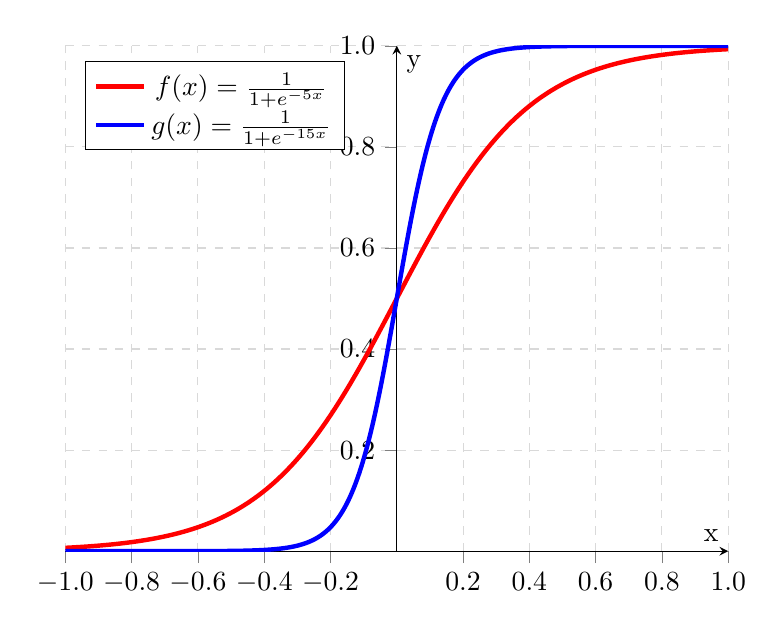
\begin{tikzpicture}
      \begin{axis}[
        legend pos=north west,
        axis x line=middle,
        axis y line=middle,
        x tick label style={/pgf/number format/fixed,
          /pgf/number format/fixed zerofill,
          /pgf/number format/precision=1},
        y tick label style={/pgf/number format/fixed,
          /pgf/number format/fixed zerofill,
          /pgf/number format/precision=1},
        grid = major,
        width=10cm,
        height=8cm,
        grid style={dashed, gray!30},
        xmin=-1,
        xmax= 1,
        ymin= 0,
        ymax= 1,
        xlabel=x,
        ylabel=y,
        tick align=outside,
        enlargelimits=false]
        % plot the stirling-formulae
        \addplot[domain=-1:1, red, ultra thick,samples=500] {1/(1+exp(-5*x))};
        \addplot[domain=-1:1, blue, ultra thick,samples=500] {1/(1+exp(-15*x))};
        \addlegendentry{$f(x)=\frac{1}{1+e^{-5x}}$}
        \addlegendentry{$g(x)=\frac{1}{1+e^{-15x}}$}
      \end{axis}
    \end{tikzpicture}
\end{itemize}

\end{document} 
